\documentclass[12pt]{article}

\usepackage[margin=1in]{geometry}
\usepackage{amsmath, amsthm}
\usepackage{amssymb}
\usepackage{graphicx}
\usepackage{times}
% \usepackage{subcaption}
\usepackage[colorlinks=true, linkcolor=black, citecolor=black, urlcolor=black]{hyperref}


\title{CSCI 5352: Homework 3}
\author{
    Zachary Caterer$^{1,2,3}$ \\
    \small $^1$Department of Computer Science, University of Colorado Boulder \\
    \small $^2$Department of Chemical and Biological Engineering, University of Colorado Boulder \\
    \small $^3$Interdisciplinary Quantitative Biology Program, University of Colorado Boulder
}
\date{\today}

\begin{document}

\maketitle

\subsection*{Collaborators}
I worked with the following people on this assignment:

\begin{itemize}
    \item Ben Braun
    \item Logan Barrios
    \item Luis Paez
    \item Michael Luzadder
    \item Pedro Lemos
\end{itemize}

\section*{Problem 1}

\subsection*{Part A}

\begin{figure}[h] 
    \centering 
    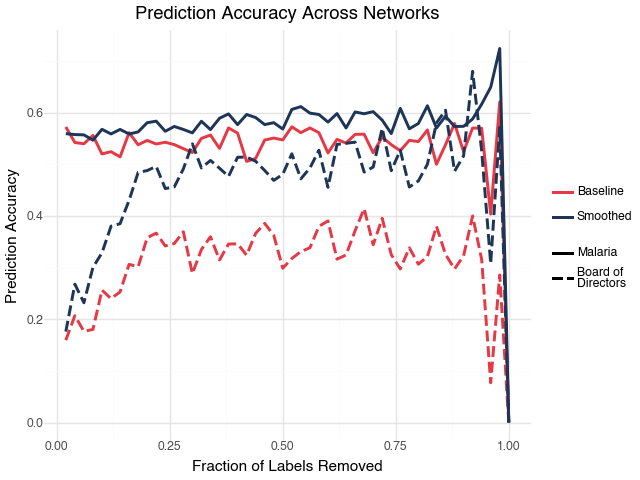
\includegraphics[width=0.95\textwidth]{../figures/combined_plot.png} 
    \caption{Prediction accuracy as a function of $\alpha$ for the Norwegian Board of Directors and Malaria var DBLa HVR networks. The solid lines represent the accuracy of the Board of Directors network, while the dashed lines represent the accuracy of the Malaria network. The red line indicates the accuracy of the baseline prediction algorithm, while the black line represents the accuracy of the local smoothing heuristic.} 
    \label{fig:Prediction_accuracy} 
\end{figure}

Figure \ref{fig:Prediction_accuracy} illustrates the prediction accuracy for the Norwegian Board of Directors and Malaria var DBLa HVR networks as a function of $\alpha$, the fraction of observed node labels. The solid lines correspond to the Malaria network, while the dashed lines represent the Board of Directors network. The red line indicates the accuracy of the baseline prediction algorithm, whereas the black line shows the accuracy of the local smoothing heuristic. Across both networks, the local smoothing heuristic consistently outperforms the baseline predictor for most values of $\alpha$. However, there are occasional points where the baseline and heuristic algorithms achieve comparable accuracy, or where the baseline slightly surpasses the heuristic due to random fluctuations in label distributions. For both networks, prediction accuracy generally increases as $\alpha$ approaches 1.0, with a notable peak just before full label observability. Interestingly, accuracy tends to dip slightly around $\alpha \approx 0.9$ before reaching its maximum. This suggests that while more observed labels typically improve performance, certain structural properties of the networks may cause minor fluctuations in predictive accuracy at high $\alpha$ values. Comparing the two networks, the Malaria network achieves consistently higher accuracy than the Board of Directors network across most $\alpha$ values. Specifically, at higher values of $\alpha$, the Malaria network reaches an accuracy of approximately 0.8, whereas the Board of Directors network attains around 0.6. Meanwhile, the baseline predictor achieves an accuracy of approximately 0.5 for both networks, aligning with theoretical expectations. For small values of $\alpha$ (e.g., $\alpha \in [0, 0.25]$), accuracy increases gradually before stabilizing in the mid-range interval $\alpha \in [0.25, 0.75]$. Notably, the gap between the local smoothing heuristic and the baseline predictor is larger for the Board of Directors network than for the Malaria network. This suggests that the smoothing heuristic is particularly effective in the Board of Directors network, likely due to stronger assortative mixing in label distributions. Overall, these results reinforce the efficacy of the local smoothing heuristic in predicting missing labels and highlight differences in network structure between the two datasets. The higher accuracy of the Malaria network suggests a stronger inherent label correlation within connected nodes, whereas the Board of Directors network, despite benefiting from the heuristic, may exhibit a more complex or less assortative structure.

\subsubsection*{Expected Accuracy for Baseline Predictor}

Let $X$ be the set of possible categorical labels, and let $p_k$ denote the empirical probability of label $k$ in the observed dataset.
\begin{equation}
    \mathbb{E}[\text{ACC}] = \sum_{k \in X} p_k^2.
\end{equation}
This follows because, for a given node with true label $k$, the probability of randomly selecting $k$ from the observed labels is $p_k$.\\

\noindent For the Malaria Network, let the label distribution be $\{p_1, p_2, \dots, p_m\}$. The expected baseline accuracy is:
\begin{equation}
    \mathbb{E}[\text{ACC}_{\text{Malaria}}] = \sum_{k=1}^{m} p_k^2.
\end{equation}

\noindent Similarly, for the Board of Directors network with label distribution $\{q_1, q_2, \dots, q_n\}$, the expected accuracy is:
\begin{equation}
    \mathbb{E}[\text{ACC}_{\text{BoD}}] = \sum_{k=1}^{n} q_k^2.
\end{equation}

\noindent Figures \ref{fig:accuracy_curves_malaria} and \ref{fig:accuracy_curves_bod} illustrate the accuracy curves for the local smoothing heuristic. The baseline predictor serves as a lower bound:

\begin{itemize}
    \item In both networks, the accuracy of the local smoothing heuristic exceeds the baseline, confirming that label assortativity improves prediction.
    \item At very low $\alpha$, accuracy approaches the baseline since there is insufficient information for smoothing.
    \item In the mid-range $\alpha$, the heuristic significantly outperforms the baseline, benefiting from label homophily.
    \item At very high $\alpha$, accuracy converges to 1 as most labels are directly observed.
\end{itemize}

This analysis highlights that local smoothing leverages network structure to improve classification, particularly when a moderate number of labels are observed.


\subsection*{Part B}

\begin{figure}[h] 
    \centering 
    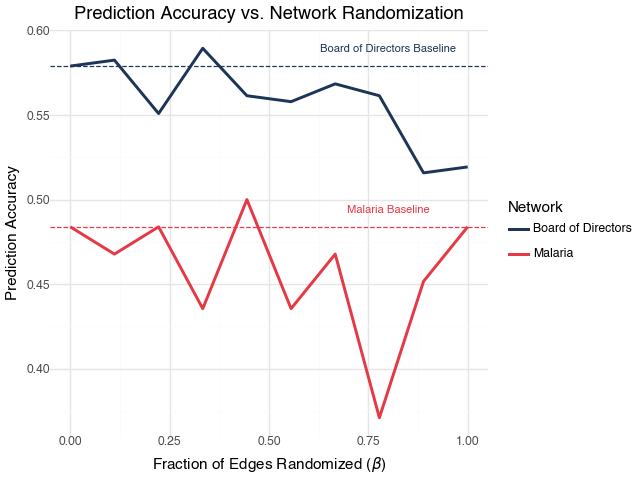
\includegraphics[width=0.95\textwidth]{../figures/accuracy_vs_randomization.png} 
    \caption{Prediction accuracy as a function of the fraction of randomized edges, $\beta$, for the Norwegian Board of Directors and Malaria var DBLa HVR networks. Solid lines represent the accuracy of the local smoothing heuristic, while dashed lines indicate the baseline accuracy. The red lines correspond to the Malaria network, and the black lines correspond to the Board of Directors network.} 
    \label{fig:accuracy_vs_randomization} 
\end{figure}

Figure \ref{fig:accuracy_vs_randomization} illustrates the prediction accuracy as a function of the fraction of randomized edges, $\beta$, for both networks. As expected, the accuracy of the local smoothing heuristic degrades toward the baseline accuracy as $\beta$ increases. This trend supports the hypothesis that as the network structure becomes increasingly randomized, the ability of the local smoothing heuristic to leverage assortative mixing diminishes. For small values of $\beta$ (i.e., when the network remains largely intact), the local smoothing heuristic significantly outperforms the baseline predictor. However, as $\beta$ increases and the network structure becomes more randomized, the accuracy steadily declines. Once $\beta$ approaches 1 (fully randomized networks), the local smoothing heuristic’s performance converges to the baseline, as expected. A key observation is that the degradation in accuracy occurs at different rates for the two networks. The Malaria network exhibits a sharper decline in performance as $\beta$ increases, suggesting that its structure is more dependent on assortative mixing patterns. In contrast, the Board of Directors network maintains a slightly higher accuracy for intermediate values of $\beta$, indicating that its node labels may be somewhat less dependent on the local connectivity structure. Additionally, the difference between the baseline and local smoothing heuristic is initially larger in the Malaria network than in the Board of Directors network. This suggests that the Malaria network initially benefits more from the local smoothing heuristic, likely due to a stronger underlying label homophily. However, as randomization increases, this advantage is quickly lost. Overall, these results highlight the extent to which the predictive power of the local smoothing heuristic relies on the empirical structure of the network. The more assortative and structured a network is, the greater the impact of randomization on predictive accuracy. Conversely, networks with less assortative mixing may be more robust to structural perturbations.

\section*{Problem 2}
\subsection*{Part A}

\begin{figure}[h] 
    \centering 
    \begin{minipage}{0.48\textwidth} 
        \centering 
        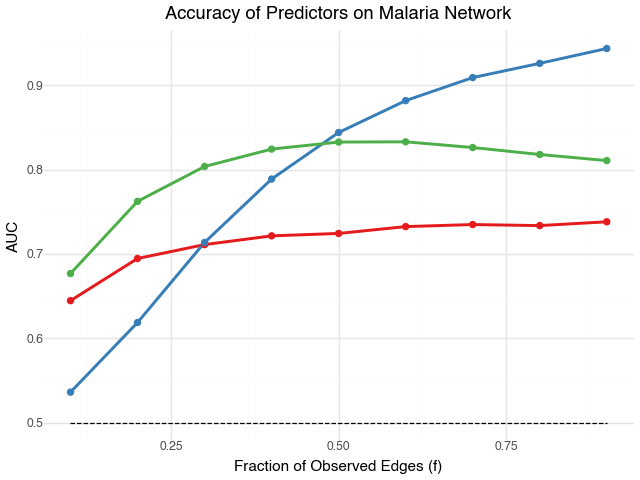
\includegraphics[width=\textwidth]{../figures/malaria_link_prediction_accuracy.png} 
    \end{minipage} 
    \hfill 
    \begin{minipage}{0.48\textwidth} 
        \centering 
        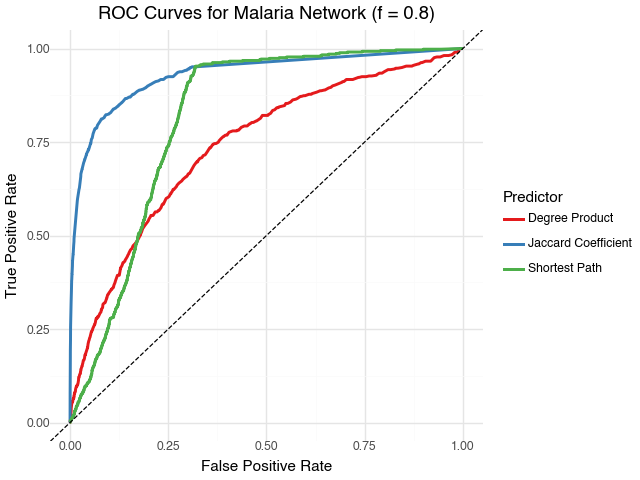
\includegraphics[width=\textwidth]{../figures/malaria_roc_curves.png} 
    \end{minipage} 
    \caption{AUC and ROC curves for the Malaria network. The left plot shows the AUC values as a function of the fraction of observed edges for three predictors, while the right plot presents the corresponding ROC curves. The predictors include Degree Product, Jaccard Coefficient, and Shortest Path. The baseline algorithm is represented by the black dashed line.} 
    \label{fig:accuracy_curves_malaria} 
\end{figure}

\begin{figure}[h] 
    \centering 
    \begin{minipage}{0.48\textwidth} 
        \centering 
        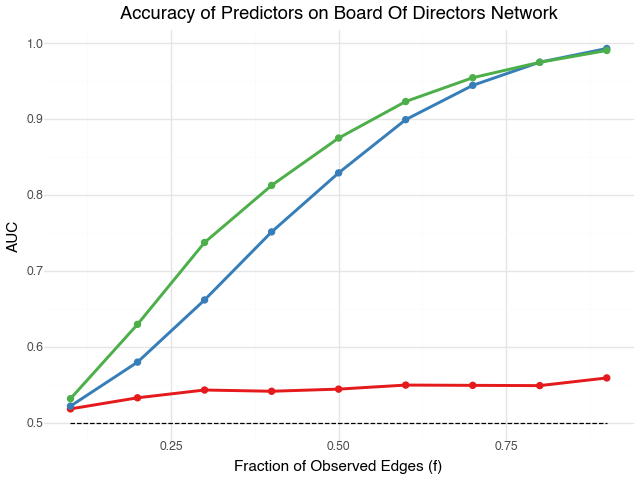
\includegraphics[width=\textwidth]{../figures/bod_link_prediction_accuracy.png} 
    \end{minipage} 
    \hfill 
    \begin{minipage}{0.48\textwidth} 
        \centering 
        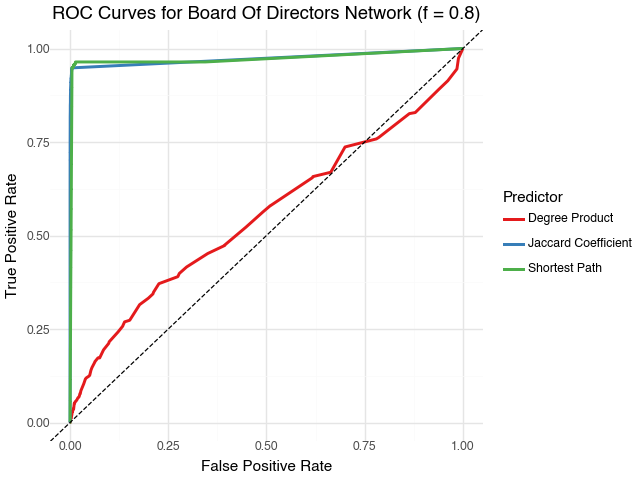
\includegraphics[width=\textwidth]{../figures/bod_roc_curves.png} 
    \end{minipage} 
    \caption{AUC and ROC curves for the Board of Directors network. The left plot shows the AUC values as a function of the fraction of observed edges for three predictors, while the right plot presents the corresponding ROC curves. The predictors include Degree Product, Jaccard Coefficient, and Shortest Path. The baseline algorithm is represented by the black dashed line.} 
    \label{fig:accuracy_curves_bod} 
\end{figure}

Figures \ref{fig:accuracy_curves_malaria} and \ref{fig:accuracy_curves_bod} display the AUC values and ROC curves for the Degree Product, Jaccard Coefficient, and Shortest Path predictors across varying fractions of observed edges. For the Malaria network, the Degree Product predictor consistently underperforms, yielding the lowest AUC values across all observed edge fractions. The Jaccard Coefficient performs best when the fraction of observed edges exceeds 0.5, while the Shortest Path predictor shows higher AUC values for lower fractions of observed edges ($f < 0.5$). In the ROC analysis, the Jaccard Coefficient provides the highest AUC, with the Shortest Path predictor following closely behind. For the Board of Directors network, the Shortest Path predictor outperforms the others across all observed edge fractions, though the Jaccard Coefficient approaches similar performance for fractions in the range $f \in [0.75,1]$. The ROC curves further support this observation, showing that the Shortest Path predictor achieves the best AUC, while the Degree Product remains close to random performance. Overall, the Jaccard Coefficient and Shortest Path predictors outperform the Degree Product predictor in both networks. However, the relative ranking of the Jaccard Coefficient and Shortest Path predictors differs between the two networks, indicating structural differences. The Malaria network benefits more from local similarity (Jaccard Coefficient), whereas the Board of Directors network is better predicted by global shortest-path relationships. The Degree Product's poor performance suggests that node connectivity alone is insufficient for accurate link prediction in these networks.

\subsection*{Part B}

This problem is extra credit, I might do if I have time. 

\begin{itemize}
    \item Discuss: (i) To what extent does the stacked model’s AUC improve upon, or not, the level-0 model AUCs? And, (ii) to what extent does the stacked model’s ROC curve improve upon, or not, the level\-0 model ROC curves?
\end{itemize}

Hint: for the training data, $c = 1000$ is a good number. However, for modest-sized networks, there may not be so many true positives; in this case, we upsample the true positives by sampling with replacement until we have $c = 1000$ examples.

\section*{Problem 3}

I read the paper ``Revisiting the Foundations of Network Analysis'' by Carter Butts. The paper addresses the fundamental question of how to appropriately choose network representations for studying complex systems. The author approached this through a conceptual and analytical framework, examining standard assumptions of network analysis while using case studies across multiple domains including biology, sociology, and communications. Through visualizations and examples, the author demonstrated how different choices in network representation - from node aggregation to edge thresholds to temporal dynamics - can significantly impact network properties and analysis outcomes. The paper's strengths lie in its clear examples from diverse fields, effective visualizations, and compelling case studies showing real-world consequences of poor representation choices, such as in HIV transmission networks.\\

\noindent However, there were opportunities for improvement and future work. The paper could have provided more specific guidelines for making network representation decisions and included more quantitative analysis of how different choices affect network metrics. Looking forward, several promising extensions are possible, including the development of formal methods for validating network representations against empirical data, creation of adaptive network representations that can change based on time scale, and integration of machine learning approaches to automatically identify appropriate levels of node aggregation. While the paper succeeds in raising awareness about the theoretical implications of network representation choices, there remains significant work to be done in developing practical tools and methods for making these choices systematically.

\end{document}